\section{KST: A Structurally Flat-Spectrum Trigger}
\label{sec:kst}

\begin{figure*}[t]
\centering
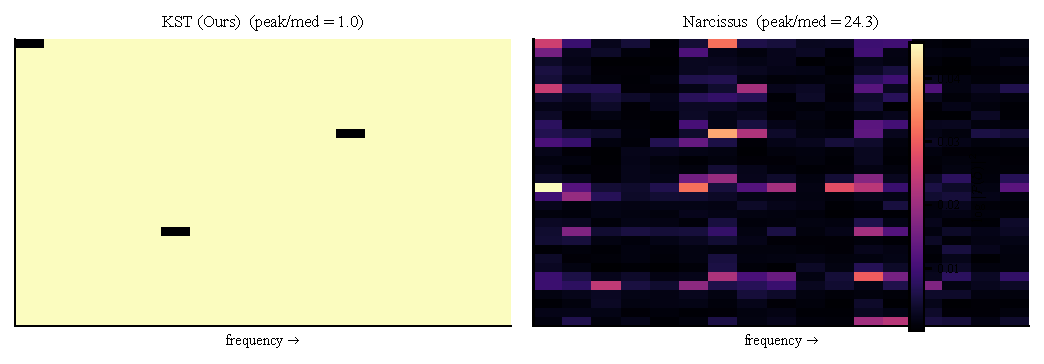
\includegraphics[width=0.85\linewidth]{floats/figures/f8_kst_spectrum.pdf}
\caption{\textbf{KST: a structurally flat-spectrum trigger.} Log magnitude of
the trigger's 2D DFT: KST spreads energy uniformly (peak/median $\approx\!1.0$)
whereas Narcissus concentrates it (peak/median $\approx\!68.9$), so KST evades
frequency-domain defenses at ASR parity.}
\label{fig:kst}
\end{figure*}

% T4 — KST flat-spectrum trigger vs references (CIFAR-10, 5% dirty-label, eps=16/255).
% Source: data_kst_eps.csv (kst_eps0.063_pr0.05_s1_result.json; narcissus_eps0.063_pr0.05_s1_result.json).
% Narcissus s-dprime computed 2026-09-16 by replaying the identical pipeline
% (same zca.pt, same KST(r=4) scorer, same xte[:2000]; KST replay reproduces 4.6433 exactly):
% script /tmp/calc_narcissus_sdprime.py, deltas resource/kst_sdt/narc_delta_eps0.0627.pt.
% BppAttack row (2026-09-16): results/kst_sdt/bppattack_q24_28_8_pr0.05_s1_result.json —
% same eval protocol (5% dirty, 300-ep ResNet-18, eval_asr), quantization 24:28:8
% (matches the SSIM~0.97 reference in docs/SATURATION-ANALYSIS.md §3; our measured
% SSIM on 256 test images is 0.954, all cells below from that single run).
% spec-peak = max/median |F(delta)|^2 (1.0 = perfectly flat).
\begin{table}[t]
\centering
\small
\begin{tabular}{l c c c c c}
\toprule
Trigger & ASR$\uparrow$ & SSIM$\uparrow$ & $\ell_2$$\downarrow$ & spec-peak$\downarrow$ & s-dprime$\uparrow$ \\
\midrule
Narcissus & 99.8 & 0.946 & 1.64 & 68.8 & 0.16 \\
BppAttack & 99.9 & 0.954 & 2.83 & $3.6{\times}10^4$ & 0.03 \\
\textbf{KST (Ours)} & \textbf{99.8} & \textbf{0.961} & \textbf{1.33} & \textbf{1.0} & 4.64 \\
\bottomrule
\end{tabular}
\caption{\textbf{KST achieves ASR parity with Narcissus while keeping the
spectrum flat} (peak/median $\approx\!1.0$ vs.\ $68.8$), at higher SSIM and lower
$\ell_2$. The flat spectrum is a structural property that defeats
frequency-domain defenses.}
\label{tab:kst}
\end{table}


Frequency-domain defenses isolate backdoors by detecting \emph{peaks} in the
trigger's DFT---Narcissus, FTrojan~\cite{wang2021ftrojan} and the triggers
of~\cite{zeng2021frequency} all concentrate energy in a few coefficients
(Narcissus: peak/median $\approx\!68.8$, Fig.~\ref{fig:kst} right). \textbf{KST}
removes that signature by construction: the trigger is parameterized by FFT
\emph{phase} only, with magnitude constrained to be constant, so its DFT
peak/median ratio is $\approx\!1.0$ (Fig.~\ref{fig:kst} left).

\paragraph{Parity ASR at higher stealth.}
At $\varepsilon\!=\!16/255$ on CIFAR-10 (dirty-label validation), KST reaches
$99.8\%$ ASR---identical to Narcissus---while being stealthier (SSIM $0.961$ vs.\
$0.946$) and smaller ($\ell_2$ $1.33$ vs.\ $1.64$, Tab.~\ref{tab:kst}). The
4th-order cumulant signature (s-dprime $4.64$) is preserved, so the trigger
remains learnable by the victim.

\paragraph{Clean-label integration.}
Plugged into the same Component-A clean-label pipeline as FAAT, KST exceeds
\emph{all} baseline triggers with the forget selection
($86.8\%$ vs.\ MultiBpp-RGB $81.2\%$) and with the res$_x$ selection
($92.6\%$ vs.\ MultiBpp-B $89.7\%$), with $\ba\!\approx\!94.7$ and a flat
spectrum throughout. KST therefore extends FAAT's stealth into the frequency
domain: where FAAT defeats \emph{spatial} defenses via $\dadapt$ and $\Lalign$,
KST defeats \emph{frequency} defenses structurally. At $\varepsilon\!=\!48$ KST
also generalizes to CIFAR-100 ($93.9\%$) and Tiny-ImageNet ($98.5\%$); the
high-confidence GTSRB regime, where KST's stealth--attack trade-off surfaces, is
analyzed in Sec.~\ref{sec:gtsrb}.
